\documentclass[12pt]{book}


\usepackage[utf8]{inputenc}
\usepackage[T1]{fontenc}
\usepackage{geometry}
\usepackage{graphicx}
\usepackage[spanish]{babel}
\usepackage{amsthm}
\usepackage{amsmath}
\usepackage{calrsfs}
\usepackage{trfsigns}

\newtheorem{thm}{Teorema}[section]
\theoremstyle{definition}
\newtheorem{dfn}{Definición}[section]
\theoremstyle{remark}
\newtheorem{note}{Nota}[section]
\theoremstyle{plain}
\newtheorem{lem}[thm]{Lema}

\geometry{letterpaper}



\title{Celdas de Combustible}
\author{Dr. Casimiro Gómez González\\
	Facultad de Electrónica, UPAEP\\
               correo: casimiro.gomez@upaep.mx\\
               Tel: 222 229 9428}
\date{Primavera 2010}

\begin{document}
\frontmatter
\maketitle


\chapter{Prólogo}

El presente material es producto del estudio realizado para diseñar celdas de combustible

\begin{flushright}

El autor\\
Casimiro Gómez González\\
Doctor en Ingeniería Mecatrónica
\end{flushright}

\tableofcontents

\mainmatter
\chapter{Introducción}
Una celda de combustible consiste de un electrodo cargado negativamente (ánodo), un electrodo cargado positivamente (cátodo), y un electrolito de membrana. El hidrógeno es oxidado en el ánodo y el oxigeno es reducido en el cátodo. 
Los protones son transportados desde el ánodo a el cátodo a través del electrolito de membrana, y los electrones son transportados a el cátodo  a través del circuito externo. 
En la naturaleza, las moléculas no pueden estar en estado iónico, por lo tanto se recombinan inmediatamente con otras moléculas para regresar a su estado neutral. 
Los protones de hidrógeno en las celdas de combustible permanecen en estado iónico viajando de molécula a molécula a través del uso de materiales especiales. Los protones 
viajan a través de la membrana de polímero hecha de ácido persulfunato con una estructura de Teflón.  Los electrones son atraídos a el material conductor y viajan a el carga 
cuando se necesita. En el cátodo, el oxigeno reacciona con protones y electrones, formando agua y produciendo calor. Tanto  el ánodo y como el cátodo contiene un catalizador
 para incrementar la velocidad del proceso electroquímico, como se muestra en la figura \ref{fig1}.

\begin{figure}
\centering
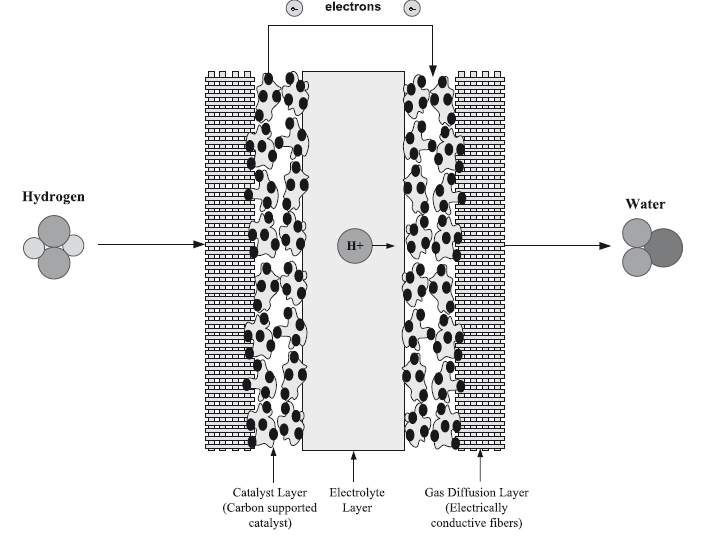
\includegraphics[width=4in]{Celdasdecombustible.png}
\caption{Configuración de una simple  Celda de combustible}
\label{fig1}
\end{figure}

Una celda de combustible típica (celda de combustible con membrana de intercambio protónico) tiene las siguientes reacciones:


\begin{align*}
Anodo: & H_2 (g) \rightarrow 2 H^{+}(aq)+2 e^{-} \\
Catodo: & \frac{1}{2} O_2 (g) + 2 H^{+}(aq)+2 e^{-} \rightarrow H_{2} O (l) \\
Total: & H_2(g) + \frac{1}{2} O_2 (g) \rightarrow H_{2}O (l)+ Energía Eléctrica+calor 
\end{align*}


Los reactantes son transportados por difusión y/o convección a la superficie  catalizada del electrodo donde las reacciones electroquímicas se realizan. El agua y el calor 
generados por la celda de combustible deben ser continuamente removidos y pueden se un tema muy importante en el comportamiento de la celda de combustible.

La pila básica de celdas de combustible PEM consiste de una membrana de intercambio protónico (PEM), capas de  catalizador y  capas de difusores de gas, placas de flujo de 
campo, juntas y placas de extremo. Esta compuesta de los siguientes elementos:

\begin{itemize}
\item \textbf{Membrana de Intercambio Protónico}.- La cual permite que los protones de Hidrógeno viajen del ánodo al cátodo y esta compuesta por una Membrana ácida de Persulfatos (nafion 112, 115, 117).
\item \textbf{Capas de catalizador}.- Rompe el combustible en protones y electrones. Los protones se combinan con el oxidante para formar agua en el cátodo de la celda de combustible. Los electrones viajan a la carga. Los catalizadores son de Platino/carbón.
\item \textbf{Capas del difusor de gas}.- Permite el combustible/oxidante viajar a través de las capas porosas, mientras se colectan electrones. Esta formado por paños de carbón o papel Toray.
\item \textbf{Placas de flujo de campo}.- distribuye el combustible y el oxidante a la capa de difusión de gas. Esta hecho de grafito, o de acero inoxidable.
\item \textbf{Juntas}.- Evitar fugas de combustible y ayuda a distribuir la presión uniformemente. Esta hecha de silicón, o Teflón.
\item \textbf{Placas de terminación}.- Mantiene las capas de la pila en su lugar. Están hechas de acero inoxidable, grafito, polietileno, y PVC.
\end{itemize}

Algunas ventajas de los sistemas de celdas de combustible son las siguientes:

\begin{itemize}
\item Las celdas de combustible tienen el potencial de operar con una alta eficiencia
\item Hay muchos tipos de fuentes de combustible y métodos para suministrar combustible a la celda de combustible.
\item Las celdas de combustible tienen un diseño altamente escalable.
\item Las celdas de combustible no producen contaminación
\item Las celdas de combustible tiene un mantenimiento bajo porque no tiene partes móviles
\item Las celdas de combustible no necesitan ser recargables, y proporcionan energía instantáneamente cuando se proporciona el combustible.
\end{itemize}

\section{Breve descripción histórica}

A William Grove se le reconoce el invento de la primera celda de combustible en 1839. Las celdas de combustible no fueron muy investigadas durante los 1800 y principios de 
los 1900s. 
Las investigaciones exhaustivas comenzaron durante 1960 en la NASA. 
Durante la última década, las celdas de combustible han sido investigadas exhaustivamente y están cada vez más cerca de la comercialización. 
A continuación se presenta un breve resumen histórico.

\begin{itemize}
 \item En 1800, W. Nicholson y A. Carlisle describieron el proceso de utilizar la electricidad para romper las moléculas del agua
 \item En  1836, William Grove demuestra el funcionamiento de una celda de combustible
 \item En 1889, Equipos separados: L. Mond y C. Langer/ C. Wright y C. Thompson/L. Cailleteton y L. Colardeau realizaron varios experimentos con celdas de combustible.
 \item En 1893, F. Ostwald describe las funciones de los componentes de las celdas de combustible.
 \item En 1896, W. Jacques construye una batería de carbon.
 \item A principios de 1900, E. Baur y sus estudiantes realizaron experimentos con dispositivos a altas temperaturas.
 \item En 1960, T. Grubb y L. Niedrach inventaron la tecnología PEMFC en General Electric.
 \item Desde 1990 hasta el presente, las investigaciones de celdas de combustible han sido intensivas en todos los tipos de celdas de combustible.
\end{itemize}

El proceso de utilizar electricidad para romper las moléculas de agua en hidrógeno y oxigeno
(electrólisis) fue descrito por primera vez en 1800 por William Nicholson y Anthony Carlisle. William
Grove inventó la primera celda de combustible en 1839, usando la idea de Nicholson y Carlisle
para ``recomponer agua''. El realizó esto combinando electrodos en un circuito en serie,
con electrodos de platino separados en oxigeno e hidrógeno, sumergidos en un electrolito que es 
una solución de ácido sulfúrico diluido. La batería de gas, o Celda Grove, generaba 12 amp de
corriente y cerca de 1,8 volts.
La NASA investigo la tecnología de celdas de combustible tipo PEM para el proyecto Gemini a inicios
del programa espacial de los Estados Unidos. Las baterías fueron usadas para los proyectos
anteriores de las misiones Mercurio, pero el proyecto Apolo necesitaba una fuente de poder
mayor y que durara un periodo de tiempo mayor. Desafortunadamente, las primeras celda de combustible
tipo PEM tenian dificultades con la contaminación interna y el filtrado de oxigeno a 
a través de la membrana. General Electric rediseño su celda de combustible, y el nuevo
modelo se comporto adecuadamente por el resto de los vuelos de el Gemini. Los diseñadores 
del proyecto Apolo y los transbordadores espaciales últimamente han escogido las celdas 
de combustible alcalinas.

General Electric continuo trabajando en celdas de combustible tipo PEM en los 70s, y diseño
la tecnología de electrolisis por PEM, la cual proporcionó a la naval de US plantas 
generadoras de oxigeno. La real naval Británica uso celdas de combustible PEM a principios
de los 80s para su flota submarina y durante la década pasada, las celdas de combustible 
tipo PEM han sido investigadas extensivamente por compañías comerciales para transporte, 
aplicaciones estacionarias y aplicaciones de potencia portátiles.


\section{Modelos matemáticos}

Los modelos matemáticos recientes para las celdas de combustible tienen las siguientes características:

\begin{enumerate}
\item  \textbf{Número de dimensiones}.- Las ecuaciones que describen la física pueden ser de una dos o tres dimensiones.
\item \textbf{Variable tiempo}.- Considerando el comportamiento o no la variable de tiempo pueden ser modelos estáticos y dinámicos
\item  \textbf{Por la cinética del ánodo y el cátodo} .- Se consideran dos modelos principales: Las ecuaciones cinéticas tipo Tafel y las ecuaciones cinéticas tipo Butler-Volmer.
\item  \textbf{Fase del ánodo y del cátodo}.- Se pueden considerar en fase gaseosa, líquida o una combinación de ambas.

\item  \textbf{Transporte de masa (ánodo y cátodo)}.- Los modelos se pueden basar en la difusión efectiva de Fick, en el modelo Nernst-Planck, en el modelo Nernst-Planck+Schlogl y tambien en el modelo Maxwell-Stefan.

\item  \textbf{Transporte de masa (Electrolito)} Los modelos se basan en Nernst-Planck+ Schlogl, o en el modelo Nernst-
Planck + coeficiente de arrastre o en el modelo Maxwell-Stefan, o bien en  la difusión efectiva de Fick.

\item \textbf{Humedecimiento de la membrana}.- Aquí los modelos utilizados con termodinámicos o empíricos

\item \textbf{Balance de energía}.- Balance de energía completo o isotérmico \cite{Mase1999} .
\end{enumerate}


\chapter{Análisis Termodinámico}
La termodinámica es el estudio de los cambios de energía desde un estado a otro. Las prediccciones
que se pueden hacer usando las ecuaciones termodinámicas son esenciales para entender
y modelar el comportamiento de las celdas de combustible desde como las celdas de combustible
transforman la energía química en energía eléctrica. Los conceptos termodinámicos 
básicos permiten predecir el estado del sistema de la celda de combustible. 

\section{Entalpia}
Cuando analizamos sistemas termodinámicos, la suma de la energía interna ($U$) y el 
producto de la presión y el volumen aparecen frecuentemente esto ha sido denominado 
``Entalpia'' ($H$) y se representa por:

 \begin{equation}
\label{equ300}
  H=U+pV
 \end{equation}
Los valores para la energía interna y entalpia pueden obtenerse de tablas termodinámicas
donde la temperatura y la presión son conocidas. Cuando analizamos mezclas de líquido
vapor en dos fases (como en las celdas de combustible), la energía interna específica
y la entalpía específica se pueden calcular utilizando las ecuaciones \ref{equ301} y 
\ref{equ302}, respectivamente.

\begin{equation}
 \label{equ301}
u = (1-x) u_f+x u_g=u_f+x(u_g-u_f)
\end{equation}

\begin{equation}
 \label{equ302}
h = (1-x) h_f+x h_g=h_f+x(h_g-h_f)
\end{equation}

\subsection{Ejemplo 2-1: Calculando la entalpía del agua}

Suponiendo agua con una presión de 1psi y a una temperatura de 100 C.

(a) Calcular la entalpia.

Buscando en tablas para la presión y la temperatura indicadas: $v=1.696 m^3/kg$ y 
$u=2506.7 kJ/kg$ entonces, sustituyendo en \ref{equ300}
\begin{equation}
 H = 2506.7 \frac{kJ}{kg}+(6894.76 \frac{N}{m^2})(1.696 \frac{m^3}{kg})(\frac{1 kJ}{10^3 N m})
\end{equation}
\begin{equation}
 H=2518.4 \frac{kJ}{kg}
\end{equation}

Se considera que $1 psi = 6894.76 N/m^2$.

(b) Si el agua es calentada a $80 C$, calcular la entalpia con una enegía interna 
específica de $400 kJ/kg$.

Revisando las tablas termodinámicas, la energía interna proporcionada esta entre los valores 
de $u_f$ y $u_g$ a $80C$, de tal forma,  que el estado del agua en una mezcla líquido-vapor.
La calidad de la mezcla se puede obtener de la ecuación \ref{equ301}:

\begin{equation}
 x = \frac{u-u_f}{u_g-u}=\frac{400-334.86}{2482.2-400}=0.0313
\end{equation}

Con los valores obtenidos por tablas,

\begin{equation}
 h = (1-x) h_f + x h_g= (1-0.0313)*334.91+0.0313*2643.7= 407.14 \frac{kJ}{kg}
\end{equation}


La entalpia de formación para una sustancia es la cantidad de calor absorbida 
o liberada cuando una mol de la sustancia es formada a partir de sustancias 
elementales en el estado de referencia. La entalpia de las sustancias en su estados 
de ocurrencia natural es definido como cero en el estado de referencia (el estado de 
referencia es típicamente considerado a $T_{ref}=25 C$ y $P_{ref}= 1 atm$). Por ejemplo, 
el hidrógeno y oxígeno en sus estados de referencia son moléculas diatómicas ($H_2$ y 
$O_2$) y de esta forma, la entalpía de formación para el $H_2$ y $O_2$ a a $T_{ref}=25 C$ y $P_{ref}= 1 atm$
es igual a cero. La entalpía de formación es típicamente determinada por mediciones de
laboratorio, y puede ser encontrada en tablas termodinámicas.

\section{Calor Específico}

Otra propiedad importante en la termodinámica y el estudio de la celdas de combustible
son las de calor específico- el cual es muy útil cuando se usa el modelo de gas ideal. El
calor específico (o capacidad calorífica) puede ser definido para sustancias puras, y
comprensibles como la derivada parcial de $u(T, v)$ y $h(T, p)$:

\begin{equation}
 \label{equ303}
c_v = \left. \frac{\partial u}{\partial T}\right|_v
\end{equation}

\begin{equation}
 \label{equ304}
c_p = \left . \frac{\partial h}{\partial T} \right|_p
\end{equation}

donde $v$ y $p$ son variables que son mantenidas constantes cuando se realiza la 
diferenciación. $c_v$ es una fucnión de $v$ y $T$, y $c_p$ es una función de $T$ y $p$. El
calor específico esta disponible es muchas tablas termodinámicas. El cociente de los calores 
específicos es llamado coeficiente de calor específico ($k$), y se puede definir:


\begin{equation}
 \label{equ305}
k = \frac{c_p}{c_v}
\end{equation}

Los valores para $v$, $u$, y $h$ pueden ser obtenidos en estado líquido usando los 
datos para líquido saturado. Para simplificar los calculos que involucran solidos
y líquidos, el volumen especìfico se supone normalmente constante y la energía interna 
específica se supone que varía solamente con la temperatura. Cuando una sustancia 
es definida de esta manera, es llamada ``incomprensible''. Porque los valores para 
$v$, $u$ y $h$ varia solo ligeramente con cambios en la presión a temperatura constante,
los siguiente se puede suponer en la mayoria de los calculos de ingeniería:
\begin{equation}
 \label{equ306}
v(T,p) \approx v_f(T)
\end{equation}

\begin{equation}
 \label{equ307}
u(T,p) \approx u_f(T)
\end{equation}

De esta forma, sustituyendo \ref{equ306} y \ref{equ307} en la ecuación \ref{equ300}, y 
despues de derivar:

\begin{equation}
 \label{equ308}
h(T,p)=u_f(T)+p v_f (T)=h_f (T)+ v_f(T)(p-p_{sat}(T))
\end{equation}

Cuando una sustancia es modelada como incompresibles, los calores específicos se suponen
iguales $c_p = c_v$. Los cambios es la energía interna específica y en la entalpia 
específica entre dos estados son funciones de la temperatura y pueden ser calculados usando
el calor específico a una temperatura constante:

\begin{equation}
 \label{equ309}
u_2-u_1= \int_{T_1}^{T_2} c_p(T) dT
\end{equation}

\begin{equation}
 \label{equ310}
h_2-h_1= \int_{T_1}^{T_2} c_p(T) dT +v(p_2-p_1)
\end{equation}

donde $c_p(T)$ es el calor específico a presión constante.

Las relaciones entre Temperatura/Presión/volumen específico para gases en muchos estados
pueden ser aproximados por las leyes de gases ideales:

\begin{equation}
 \label{equ311}
p v = R T
\end{equation}

donde $p$ es la presión, $v$ es el volumen específico, $T$ es la temperatura, y
$R$ es la constante de gas ideal. Si consideramos que $v=V/n$, obtenemos la siguiente
ecuación:

\begin{equation}
 \label{equ312}
p V = n R T
\end{equation}

Cuando el modelo de gas ideal es usado, la energía interna específica y la entalpia 
específica depende solamente de la temperatura, así:

\begin{equation}
 \label{equ313}
u_2(T_2)-u_1(T_1) = \int_{T_1}^{T_2} c_v(T) d T
\end{equation}

\begin{equation}
 \label{equ314}
h_2(T_2)-h_1(T_1) = \int_{T_1}^{T_2} c_p(T) d T
\end{equation}

Las relaciones entre el calor especìfico de los gases ideales pueden ser expresados
por:

\begin{equation}
 \label{equ315}
c_p(T) = c_v(T)+R
\end{equation}

Hay varias alternativas para las ecuaciones del calor específico. Una que es fácil
de integrar es la forma polinomial:

\begin{equation}
 \label{equ316}
\frac{c_p}{R}=\alpha + \beta T+ \gamma T^2+ \delta T^3+\varepsilon T^4
\end{equation}

Los valores para $\alpha$, $\beta$, $\gamma$, $\delta$ y $\varepsilon$ se pueden 
encontrar en muchas tablas termodinámicas y se puede encontrar en el sitio web del NIST. Usando
tablas para gases ideales, la entalpia se puede obtener a partir de:

\begin{equation}
 \label{equ317}
\Delta h_T = h_{298.15}+ \int_{298.15}^T \Delta c_p d T
\end{equation}

donde $h_{298.15}$ es la entalpia a la temperatura de referencia. El calor específico
promedio se puede aproximar como una función lienal de la temperatura:

\begin{equation}
 \label{equ318}
\overline{c_p}= c_p \left ( \frac{T+T_{ref}}{2} \right )
\end{equation}

donde $\overline{c_p}$ es el calor específico promedio a temperatura constante, $T$ 
es la temperatura dada, y $T_{ref}=25^{\circ} C$.

La entalpia de un gas seco es

\begin{equation}
 \label{equ319}
h_g = c_{pg} T
\end{equation}

donde $h_g$ es la entalpia del gas seco, $J/g$, $C_{pg}$ es el calor específico del gas,
$J/gK$ y $T$ es la temperatura en $^{\circ}C$.

Cuando tratamos con mezclas de dos fases líquido-vapor, las ecuaciones \ref{equ315} hasta
la \ref{equ319} son útiles. La entalpia del vapor de agua es

\begin{equation}
 \label{equ320}
h_v = c_{pv}t+h_{fg}
\end{equation}

donde $h_{fg}$ es el calor de evaporación, $2500 J/g$ a $0 ^\circ C$. La entalpia 
en el gas húmedo es entonces:

\begin{equation}
 \label{equ321}
h_{vg} = c_{pg} t + x(c_{pv} t + h_{fg})
\end{equation}

y las unidades son $j/g$ del gas seco.

La entalpia del agua líquida es

\begin{equation}
 \label{equ322}
h_w = c_{pw}t
\end{equation}

Si el gas contiene tanto agua como vapor, la entalpia se puede encontrar por:

\begin{equation}
 \label{equ323}
h_{vg} = c_{pg}t + x_{v}(c_{pw}t+h_{fg})+x_{w}c_{pw}t
\end{equation}

donde $x_v$ es el contenido de vapor de agua y $x_w$ es el contenido de agua líquida. El
contenido total de agua es

\begin{equation}
 \label{equ324}
x = x_v + x_w
\end{equation}

El aire que entra en la celda es generalmente  humidificado para prevenir que la membrana
cercana a la entrada de aire se seque. El aire entra a la celda relativamente seco. A 
menor temperatura, menor cantidad de agua es necesaria para humidificar la celda que a
altas temperaturas. Como el aire de la celda es calentado y la presión se incrementa, es
necesaria mas y mas agua. 

\section{Entropía}

La entropía puede se definida como la cantidad de ``desorden'' en un sistema, y se 
expresa como:

\begin{equation}
 \label{equ325}
S_2-S_1 = \left [ \int_1^2 \frac{\delta Q}{T} \right]
\end{equation}

Esto es válido para cualquier proceso reversible que enlaza dos estados. La entropía
es calculada de la misma manera que la entalpia - usando las propiedades $v$, $u$ y $h$.
Cuando tratamos con mezclas de dos fases liquido-vapor como en las celdas de combustible,
la entropía específica puede ser calculada de la misma forma que la entalpía:

\begin{equation}
 \label{equ326}
s = (1-x) s_f + x s_g = s_f + x (s_g - s_f)
\end{equation}

Como la entalpía, los valores para $v$, $u$ y $h$ varian ligeramente con los cambios
de presión a temperatura fija; por lo tanto, lo siguiente se puede suponer en la 
mayoria de los cálculos de ingeniería:

\begin{equation}
 \label{equ327}
s(T, p)=s_f(T)
\end{equation}

Cuando un sistema puro y comprensible se somete a un proceso reversible en la ausencia
de gravedad y de movimiento general del sistema, el balance de energía se puede escribir
como:

\begin{equation}
 \label{equ328}
\delta Q_{int,rev}= d U + \delta W_{int,rev}
\end{equation}
En un sistema comprensible simple, el trabajo puede ser definido como:

\begin{equation}
 \label{equ329}
\delta W_{int,rev}=p dV
\end{equation}

Sustituyendo la ecuación \ref{equ329} en \ref{equ328}, obtenemos:

\begin{equation}
 \label{equ330}
T d S = dU - p dV
\end{equation}

Otra ecuación útil se puede obtener sustituyendo en la ecuación \ref{equ300}:

\begin{equation}
 \label{equ331}
T d S = dH -V dp
\end{equation}

Aún cuando estas ecuaciones se han obtenido considerando un proceso reversible 
internamente, los cambios de entropía calculados con estas ecuaciones son válidas 
para el cambio en cualquier proceso del sistema, reversible o irreversible, entre
dos estados de equilibrio.

Cuando el modelo de gas ideal es usado, la entropía específica depende solamente de 
la temperatura y puede derivarse de las ecuaciones \ref{equ330} y \ref{equ331} por 
lo tanto:

\begin{equation}
 \label{equ332}
s_2(T_2, v_2) - s_1(T_1, v_1)=\int_{T_1}^{T_2} c_v(T) \frac{d T}{T}+R ln \frac{v_2}{v_1}
\end{equation}

\begin{equation}
 \label{equ333}
s_2(T_2, p_2) - s_1(T_1, p_1)=\int_{T_1}^{T_2} c_p(T) \frac{d T}{T}+R ln \frac{p_2}{p_1}
\end{equation}

Como la entalpía, la entropía puede obtenerse usando las tablas de gas ideal:

\begin{equation}
 \label{equ334}
\Delta s_{T} = s_{298.15}+\int_{298.15}^{T} \Delta c_p d T
\end{equation}

donde $s_{298.15}$ es la entropía a la temperatura de referencia.

\section{Cambio de la energía libre de la Reacción Química}

La conversión de los cambios de la energía libre asociados con una reacción química
directamente en energía eléctrica es debido a la conversión de energía electroquímica.
Estos cambios de la energía libre es una medida del máximo trabajo eléctrico ($W_{elec}$)
que un sistema puede realizar a una temperatura y presión constante desde la reacción. Esto
es calculado por el cambio negativo en la energía libre de Gibbs ($\Delta G$) para el
proceso, y puede expresarse en caantidades molares como:

\begin{equation}
 \label{equ335}
W_{elec}=- \Delta G
\end{equation}
 
Esta energía libre de Gibbs es la energía necesaria para un sistema a temperatura
constante con un volumen despreciable,menos cualquier energía transferida al 
ambiente debido al flujo de calor. Esta ecuación es valida a cualquier temperatura 
y presión constante para muchos sistemas de celdas de combustible. De la segunda ley
de la termodinámica, el cambio en la energía libre, o máximo trabajo utilizable,
puede se obtenido cuando una celda de combustible ``perfecta'' trabaja irreversiblemente
es dependiente de la temperatura. así, $W_{elec}$,  la potencia eléctrica de salida, es

\begin{equation}
 \label{equ336}
W_{elec}= \Delta G = \Delta H - T \Delta
\end{equation}

donde $G$ es la energía libre de Gibbs, $H$ es el calor contenido (Entalpía de 
formación), $T$ es la temperatura absoluta, y $S$ es la entropía. La enegía libre 
de Gibbs es igua a la entalpía si el cambio de entropía es cero. Como se puede ver 
por la definición de la función de la energía libre de Gibbs, es una función 
decreciente con la temperatura,  pero la tendencia es complicada por la dependencia
de la temperatura tanto de la entalpía como de la entropía. El termino $T \Delta S$ 
crece más rápido incrementando $T$ que el término $\Delta H$ debido a su mayor dependencia
de la temperatura, debido a que tiene la forma $T ln (\frac{T}{T})$, mientras que
la entalpía es simplemente ($T-T$). 

El potencial de un sistema para realizar trabajo eléctrico por cambios, $Q$ (coulombs),
a través de las diferencias de potencial eléctrico, $E$ en volts, es:

\begin{equation}
 \label{equ337}
W_{elec}= E Q
\end{equation}

Si el cambio se supone que es llevado a cabo por electrones:

\begin{equation}
 \label{equ338}
Q = n F
\end{equation}
 
donde $n$ es el número de moles de electrones transferidos y $F$ es la constante
de Faraday ($96, 485$ coulombs por mol de electrones). Combinando las tres últimas
ecuaciones para calcular el máximo voltaje reversible proporcionado por la celda:

\begin{equation}
 \label{equ339}
\Delta G = - n F E_r
\end{equation}

donde $n$ es el número de moles de electrones transferidos y $F$ es la constante
de Faraday, y $E_r$ es el potencial estandar reversible.

Las relaciones entre el voltaje y temperatura es derivada tomando la energía libre,
linealizando alrededor de las condiciones estandar de $25^{\circ} C$, y asumiendo que los
cambios de entalpía $\Delta H$ no cambia con la temperatura:

\begin{equation}
 \label{equ340}
E_r = - \frac{\Delta G}{rxn}= - \frac{\Delta H - T \Delta S}{n F}
\end{equation}

\begin{equation}
 \label{equ341}
\Delta E_r = \left( \frac{d E}{d T} \right) (T-25) = \frac{\Delta S}{n F}(T-25)
\end{equation}

donde $E_r$ es eñ voltaje reversible de estado estandar, y $\Delta G_{rxn}$ es el cambio
de la energía libre estandar para la reacción. El cambio de entropía es negativo;por lo 
tanto, el voltaje de circuito abierto disminuye con el incremento de temperatura. La
celda de combustible es teoricamente mas eficiente a bajas temperaturas. Sin embargo,
el transporte de masa y la conducción iónica son más rápidas a altas temperaturas, y
esto compensa las caidas del voltaje a circuito abierto.

Para cualquier reacción química

\begin{equation}
 \label{equ342}
j A + kB \rightarrow mC + nD
\end{equation}

Los cambios en la enegía libre de Gibbs entre los productos y ractantes es

\begin{equation}
 \label{equ343}
\Delta G = m G_c + n G_D - j G_A- j G_B
\end{equation}

En el casho de una celda de combustible de hidrógeno-oxígeno bajo condiciones de estado
estandar:

\begin{equation*}
    \begin{aligned}
      H_2 (g) + \frac{1}{2}O_2(g) \rightarrow H_2O(l)\\
      (\Delta H = -285.8 kJ/mol; \Delta G = -237.3 kJ/mol) \\
      E_{H_2/O_2}= \frac{-237.3 kJ/mol}{2 mol*96485 C/mol}=1.229 v
    \end{aligned}
\end{equation*}

A presiones y temperaturas estandar, este es el voltaje más alto obtenido
de una celda de combustible hidrógeno-oxígeno. Muchas de las reacciones
de celdas de combustible tienen voltajes en el rango de $0.8$ a $1.5$ V. Para obtener 
voltajes mas elevados, varias celdas de combustible tienen que conecta en serie.

La celdas de combustible pueden trabajar a cualquier presión, y comúnmente es una
ventaja trabajar a presiones superiores a la atamosférica. Los rangos típicos para 
las celdas de combustible son presiones atmosféricas de $6$ a $7$ bars. El cambio en 
la enegía libre de Gibbs relacionada con la presión es:

\begin{equation}
 \label{equ344}
d G = V_m dP
\end{equation}

donde $V_m$ es el volumen molar ($m^3/mol$, y $P$ es la presión en pascales. Para un
gas ideal:

\begin{equation}
 \label{equ345}
P V_m = R T
\end{equation}

Por lo tanto:

\begin{equation}
 \label{equ346}
dG = RT \frac{dP}{P}
\end{equation}

Despues de integrar:

\begin{equation}
 \label{equ347}
G=G_0 + RT ln \left( \frac{P}{P_0} \right)
\end{equation}

donde $G_0$ es la enegía libre de Gibbs a presión y temperatura estandar ($25^\circ C$
y $1$ atm), y $P_0$ es la presión estandar ($1$ atm), la cual es una forma de 
la ecuación de Nernst.

Si la ecuación \ref{equ347} es sustituida en la ecuación \ref{equ343} para cada sustancia
obtenemos:

\begin{equation}
 \label{equ348}
G= G_0 + R T ln \frac{\left ( \frac{P_C}{P_0} \right )^m \left ( \frac{P_D}{P_0} \right )^n}{\left ( \frac{P_A}{P_0} \right )^j \left ( \frac{P_B}{P_0} \right )^k}
\end{equation}

donde $P$ es la presión parcial de los reactantes o especies producto, y $P_0$ es 
la presión de referencia.

Para la reacción de una celda de combustible de hidrógeno-oxígeno, la ecuación
de Nernst es


\begin{equation}
 \label{equ349}
G = G_0 + RT ln \left (  \frac{P_{H_2} P_{O_2}^{0.5} }{P_{H_2O}} \right )
\end{equation}

Por lo tanto, el potencial de la celda como función de la temperatura y presión es:


\begin{equation}
 \label{equ350}
G = \left (  \frac{\Delta H}{n F} - \frac{T \Delta S}{n F}  \right ) + RT ln \left (  \frac{P_{H_2} P_{O_2}^{0.5} }{P_{H_2O}} \right )
\end{equation}


Para condiciones no estandar, el voltaje reversible de la celda de combustible
puede ser calculada desde el balance energético entre los reactantes y los productos.
Las ecuaciones \ref{equ351} reduce a la forma común de la ecuación de Nenst:


\begin{equation}
 \label{equ351}
E_t= E_t-\frac{RT}{nF}ln [\prod_{\substack{i}}\alpha _i^{v_i}]
\end{equation}

donde $R$ es la constante de gas ideal, $T$ es la temperatura, $\alpha _i$ es la 
actividad de la especie $i$, $v_i$ es el coeficiente estequiométrico de la especie $i$,
y $E_r$ es el voltaje reversible es estado estandar, el cual es una función de la
temperatura y presión.

La reacción de la celda de combustible de oxígeno-hidrógeno es escrita usando la
ecuación de Nernst:

\begin{equation}
 \label{equ352}
E=E_r- \frac{RT}{2F}ln \frac{a_{H_2O}}{\alpha _{H_2}\alpha _{O_2}^{1/2}}
\end{equation}

donde $E$ es el voltaje de la celda, $E_r$ es el voltaje reversible en estado estandar,
$R$ es la constante de gas universal, $T$ es la temperatura absoluta, $N$ es el
número de electrones consumidos en la reacción, $F$ es la constante de Faraday. Si
la celda de combustible esta trabajando abajo de $100^\circ C$, la actividad del
agua puede ser ajustada a $1$ porque el agua se supone en estado líquido. A presiones
absolutas de $1.00 atm$ (como a nivel del mar en un dia normal), con una concentración 
efectiva de $1.00$ mol de $H^+$ por litro de el ácido electrolitro, la razón de
$1.00^{1/2}:1.00=1$, y $ln 1=0$. Por lo tanto $E=E_r$. El potencial estandar del 
electrodo es realizado cuando los productos y reactantes estan en sus estados estandar.

A temperatura y presión estandar, el potencial teórico de una celda de combustible 
hidrógeno-aire puede ser calculado como sigue:

\begin{equation}
 \label{equ353}
E=1.229 - \frac{8.314(J/(mol*K))*298.15}{2*96485(C/mol)}ln \frac{1}{1*0.21^{1/2}}=1.219 V
\end{equation}

El potencial entre el catodo de oxígeno donde la reducción ocurre y el ánodo de hidrógeno
en donde la oxidación ocurre será de 1.229 V a condiciones estandares cuando no fluye 
corriente. Cuando una carga se conecta a los dos electródos, la corriente fluirá 
conforme halla una reacción entre el hodrógeno y oxígeno. Si la corriente es
pequeña, la eficiencia de la celda (medida en voltaje) puede ser mayor que 0.9 V,
con uma eficiencia mayor que $90\%$. Esta eficiencia es mayor que los complejos 
sistemas de las máquinas térmicas, los cuales pueden alcanzar una eficiencia máxima
del $60\%$.

Suponiendo que los gases son ideales (la actividad de los gases son iguales a sus presiones
parciales, y la actividad del agua es igual a la unidad), la ecuación \ref{equ351} se 
puede reescribir:

\begin{equation}
 \label{equ354}
E_t = E_r -\frac{RT}{nF}ln [\prod_{\substack{i}}\left ( \frac{p_i}{p_0} \right )^{v_i}]
\end{equation}

donde $p_i$ es la presión parcial de especies $i$, y $p_0$ es la presión de 
referencia. Para gases ideales o para estimaciones de gases no ideales, la presión
parcial de las especies $A$, $p_A^*$ puede ser expresada como un producto de la 
presión total $P_A$ y la fracción molar $x_A$ de las especies:

\begin{equation}
 \label{equ356}
p_A^* = x_A P_A
\end{equation}

Si la fracción molar de el combustible es desconocida, puede ser estimada tomando 
el promedio de las condiciones de entrada y salida:

\begin{equation}
 \label{equ357}
X_A = \frac{1-X_{C, ánodo}}{1+\left( \frac{X_{ánodo}}{2} \right)\left(1+ \frac{\xi _{A}}{\xi_{A-1}} \right)}
\end{equation}

donde $\xi _{A}$ es la razón de flujo estequiométrico, $X_{ánodo}$ es la razón molar 
de las especies 2:1 en gas seco, y $X_{C, ánodo}$ es:




\chapter{Modelos matemáticos de micro fluidos}
El diseño de los micro canales de una micro celda de combustible, se divide en dos secciones, la
primera realiza el estudio de los micro canales por donde circula un fluido en una sola fase, es
decir se analiza el ánodo por donde circula el metanol mezclado con agua en fase líquida. La
segunda sección estudia los micro canales del cátodo, por donde circula el aire, aquí es importante
puntualizar que en el cátodo también circula agua, debido a la reacción que allí se presenta,
además circulan pequeñas cantidades de bióxido de carbono, por lo tanto el análisis de los micro
canales para el cátodo debe considerar que hay sustancias en dos fases: el agua en fase líquida,
el aire y el bióxido de carbono el fase gaseosa.

\section{Escalamiento}

Es posible identificar los siguientes efectos de escalamiento cuando utilizamos micro canales por
los que fluye un fluido en una sola fase

\begin{enumerate}
 \item La conducción de calor axial en el fluido.
 \item La transferencia de calor entre las paredes y el fluido.
 \item La rugosidad de las paredes.
 \item La disipación viscosa.
\end{enumerate}
Para una geometría determinada de los micros canales, el flujo de calor debido a la conducción de
calor axial depende del número de Reynolds, lo cual es significativo a bajas velocidades de flujo.
Muchos estudios señalan la importancia de considerar las variaciones de las propiedades termo
físicas con la temperatura, en particular la variación de la viscosidad y la conductividad térmica,
particularmente a valores bajos del número de Reynolds; mientras que la densidad, y calor
específico se consideran independientes de la temperatura
La rugosidad de las paredes tiende a afectar el valor del factor de fricción y el valor del número de
Reynolds critico al cual el flujo pasa de ser laminar a turbulento

\section{Ecuación de Navier-Stokes para micro fluidos}

La segunda ley de Newton aplicada a fluidos se le denomina ecuación de Navier-Stokes. Esto
constituye las ecuaciones de movimiento para un campo vectorial de Euler $\mathbf{v}(\mathbf{r},t)$. Para una
partícula ordinaria de masa bajo el efecto de fuerzas externas, la segunda ley de Newton
establece

\begin{equation}
\label{equ200}
 m d_t \mathbf{v}= \sum_{j} \mathbf{F}_j
\end{equation}

En Mecánica de fluidos se toma un volumen de fluido como partícula cuya densidad es $\rho$ y la densidad de fuerza es $\mathbf{f}_j$

\subsection{Derivada material}

Sea un campo vectorial de las velocidades de un fluido $\mathbf{\upsilon}= \mathbf{\upsilon}(x(t), y(t), z(t), t )$ y consideramos 
la aceleración de una partícula en el fluido $a = \frac{d \upsilon}{d t}$. Si aplicamos la regla de la cadena obtenemos,

\begin{equation}
 \label{equ201}
\mathbf{a}(t) = \frac{d \upsilon}{d t} =  \frac{\partial \upsilon}{\partial x} \frac{d x}{d t} +  \frac{\partial \upsilon}{\partial y} \frac{d y}{d t} +  \frac{\partial \upsilon}{\partial z}\frac{d z}{d t}+\frac{\partial \upsilon}{\partial t}\frac{d t}{d t}
\end{equation} 

Simplificando la notación tenemos

\begin{equation}
 \label{equ202}
(\mathbf{a}(t))_i = \frac{\partial \upsilon_i}{\partial x_j} \frac{d x_j}{d t} + \frac{\partial \upsilon}{\partial t}\frac{d t}{d t}=\frac{\partial \upsilon_i}{\partial x_j} \frac{d x_j}{d t} + \frac{\partial \upsilon}{\partial t}
\end{equation} 


\bibliographystyle{apalike} %% plain.bst
\bibliography{../cashoBibliografoa.bib}


\backmatter
\end{document}
